\chapter{Testdurchführungen}
\label{chap:Testphasen}

Es wurden im Rahmen dieser Arbeit eine grosse Anzahl an Messungen und Testfällen durchgeführt. 
Die Testkonzepte im digitalen Anhang \ref{AnhangE} geben detailliert Auskunft über die Testdurchführung. 
Nachfolgende Grafik zeigt 

\section{Messinstrumente}

Für die Messungen wurde das Panasonic AMG8834 Eval Kit verwendet. Es bietet den Vorteil, dass sich, dank einem Atmel Prozessor und einer bereits vorhandene Software, die Sensordaten als Rohdaten über USB bzw. UART mit dem Programm H-Term auslesen lassen. 
Das erstellten Programm ConvertValue\_V2\footnote[12]{im digitalen Anhang bereitgestellt} wandelt die Rohdaten in \ac{CSV}-Files um, damit diese mit Matlab und Python verwendet werden können.

Zudem können die Daten zur Echtzeit über Bluetooth an die zur Verfügung stehende App übermittelt werden, damit die Messungen zur Echtzeit verbalisierbar sind.

Zur Verifizierung der Messwerte das digitale Thermometer Fluke 52-II und die Wärmebildkamera Fluke TI 125 verwendet.

\section{Grundlagenmessungen}

Die Grundlagenmessungen geben Auskunft über die Eigenheiten des Messprinzips. Dabei wurde einerseits physikalische Aspekte, welche im vorherigen Kapitel erläutert wurden verifiziert und weitere.
Die nachfolgenden Unterkapitel sind Abschnittsweise in Fragestellung, Vorgehen und Resultate gegliedert.


\subsection{Streuung}

\textbf{Fragestellung:} Um eine Person zu detektieren, benötigt es eine Temperaturdifferenz zwischen dem Hintergrund und der Person. Daher stellt sich die Frage wie gross die Streuung des Sensor ist. Diese Streung gibt die minimale Differenz vor, damit die Person auch bei Streuwerten unterschieden wird.

\textbf{Vorgehen:} In einem 60-minütigen Messdurchgang bei konstanter Umgebungstemperatur von 22.6°C wurde eine konstant 22.6°C Oberfläche ausgemessen. In Abbildung \ref{fig:temperaturverhalten} sind die Thermistorwerte(\textcolor{blue}{blau}) und die Pixelwerte(Werte zwischen \textcolor{red}{rot} \& \textcolor{orange}{orange}) dargestellt.
\begin{figure}[H]
	\centering
	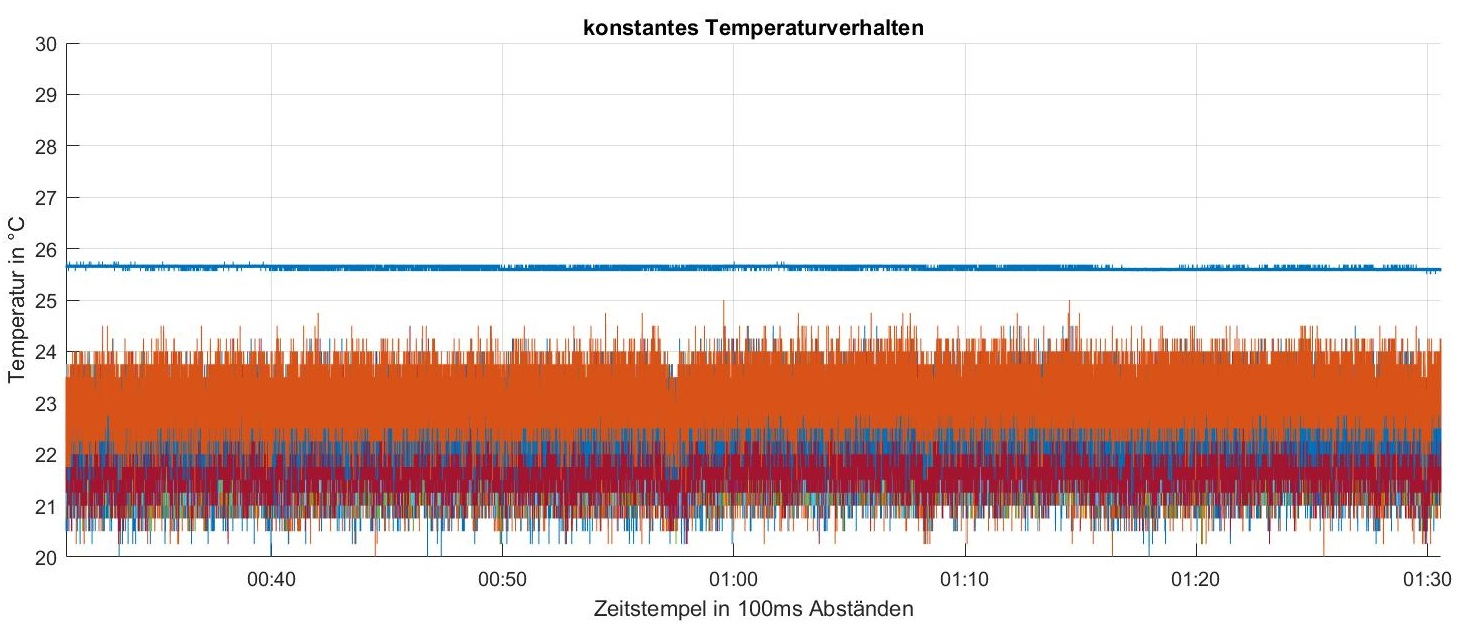
\includegraphics[width=1.0\textwidth]{fig/Temperaturverhalten}
	\caption[konstantes Temperaturverhalten]{konstantes Temperaturverhalten}
	\label{fig:temperaturverhalten}
\end{figure}

\textbf{Ergebnisse:} Es fällt auf, dass die Thermistorwerte entgegen den Erwartungen eine höhere Temperatur (26°C anstelle 22.8°C) aufweist. Es wurden mehrere Eval Kits ausgetestet und es konnte kein konstanter Offset eruiert werden. Es ist von Exemplarstreuungen auszugehen. Die Thermistorwerte sind im Allgemeinen um mehrere Grad höher als die gemessenen Werte. 

Zusätzlich ist in der Abbildung \ref{fig:temperaturverhalten} ersichtlich, dass die Temperaturwerte der einzelnen Pixel nicht auf gleichen Niveau liegen. die Pixelreihe \textcolor{orange}{orange} streut um 23°C, wobei die Pixelreihe \textcolor{red}{rot} deutlich tiefer liegt. Daher kann im Allgemein nicht davon ausgegangen werden,  


\begin{figure}[H]
	\centering
	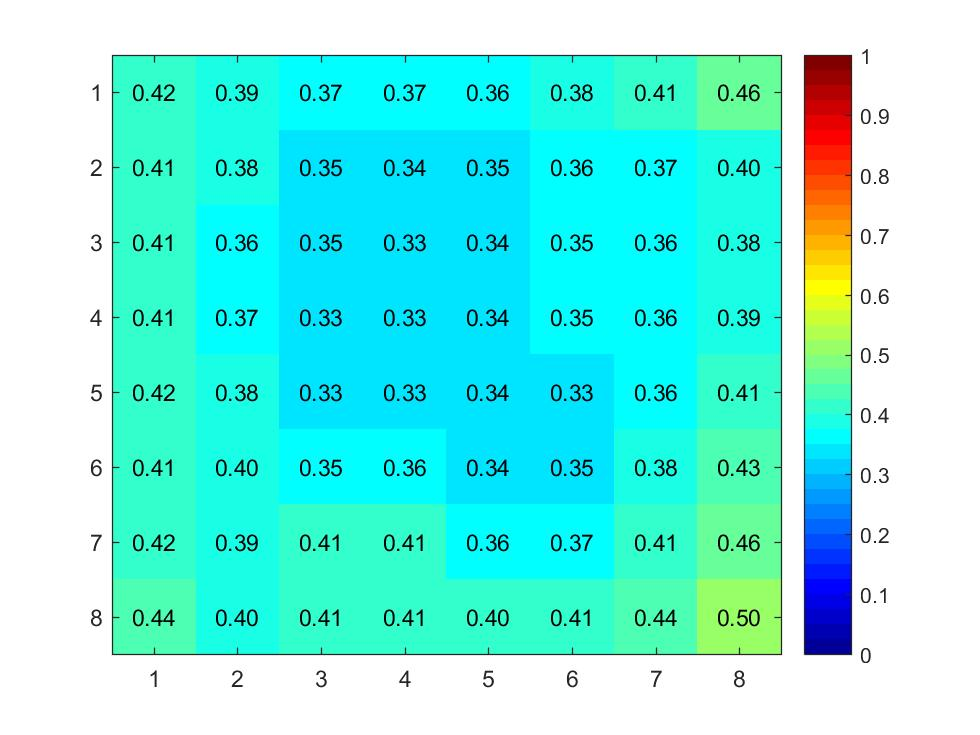
\includegraphics[width=0.5\textwidth]
	{fig/Distanz_140cm_std_.jpg}
	\caption[Streuung der einzelnen Pixel im Vergleich]{Streuung der einzelnen Pixel im Vergleich}
	\label{fig:Streuung}
\end{figure}


\subsection{Einflussfaktor Infrarotstrahlung}



\subsection{Temperaturverhalten im Aussenbereich}


\subsection{Temperaturverhalten im Aussenbereich}



\begin{figure}[H]
	\centering
	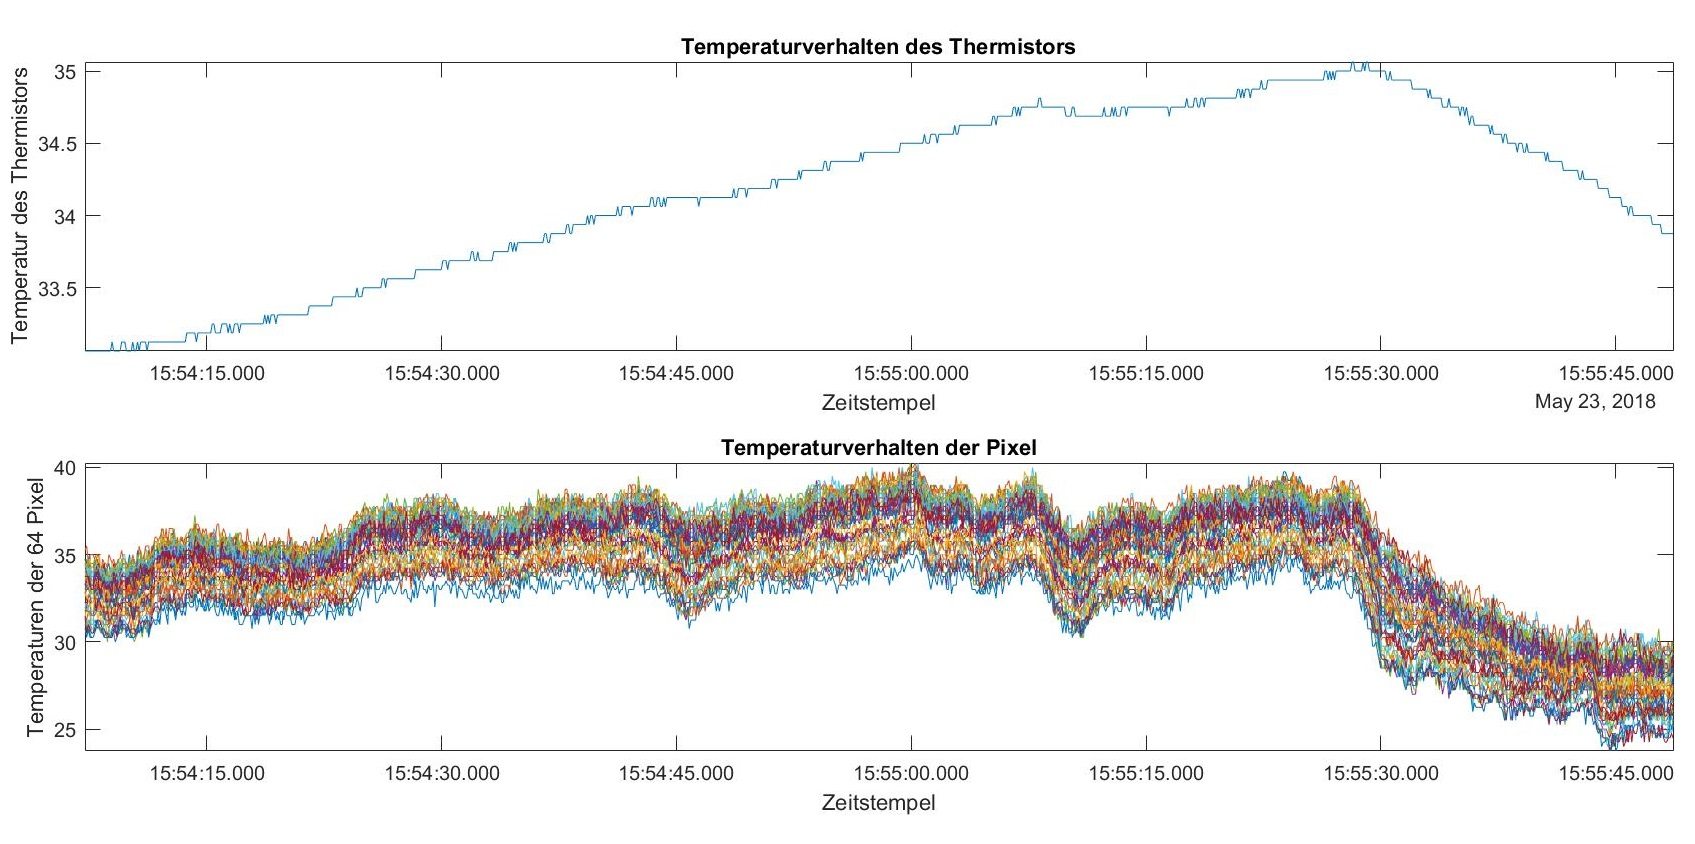
\includegraphics[width=1.0\textwidth]{fig/Temperaturverhalten2}
	\caption{}
	\label{fig:temperaturverhalten2}
\end{figure}


\subsection{Einfluss Störquellen}

Dieser Abschnitt befasst sich mit den Einfluss von externen Quellen auf den Sensor. Dabei spielen natürliche Einwirkungen wie Luftströme, Umgebungstemperaturen und Lichtquellen einen enormen Einfluss. 



Weitere Störquellen sind Objekte, welche sich innerhalb des \ac{FOV} des Sensors befinden. In Abbildung 26 ist eine



Neben natürlichen Störquellen und Objekten besteht ein enormer Unterschied bei der Bekleidung der zu messenden Personen. 




\section{Personenmessungen}
Bei der Personenmessungen wurden unterschiedliche Probanden in einem Aufzug ausgemessen auf dessen Wärmestrahlung analysiert. 

\subsection{Fragestellung}




\subsection{Vorgehen}
Dabei standen insgesamt 6 Probanden zur Verfügung. Die Probanden wurden entsprechend ihrer Grösse und dem Körperumfang in die Kategorien klein [k], mittel [m] und groß [g] unterteilt. Nachfolgende Tabelle gibt über die Masse der Probanden Auskunft. 

\begin{table}[H]
\centering
\caption{Masse der Probanden}
\label{my-label}
\begin{tabular}{|
		>{\columncolor[HTML]{C0C0C0}}c |c|c|c|c|}
	\hline
	& \cellcolor[HTML]{C0C0C0}\textbf{Grösse {[}cm{]}} & \cellcolor[HTML]{C0C0C0}{\color[HTML]{333333} \textbf{Breite {[}cm{]}}} & \cellcolor[HTML]{C0C0C0}{\color[HTML]{333333} \textbf{Tiefe {[}cm{]}}} & \cellcolor[HTML]{C0C0C0}\textbf{Kategorie} \\ \hline
	\textbf{Proband 1} & 162                                              & 46                                                                      & 28                                                                     & k                                          \\ \hline
	\textbf{Proband 2} & 166                                              & 52                                                                      & 33                                                                     & k                                          \\ \hline
	\textbf{Proband 3} & 167                                              & 48                                                                      & 25                                                                     & k                                          \\ \hline
	\textbf{Proband 4} & 172                                              & 53                                                                      & 34                                                                     & m                                          \\ \hline
	\textbf{Proband 5} & 175.5                                            & 54                                                                      & 34                                                                     & m                                          \\ \hline
	\textbf{Proband 6} & 185.5                                            & 63.5                                                                    & 42                                                                     & g                                          \\ \hline
\end{tabular}
\end{table}
\subsection{Messaufbau}

Für den Messaufbau wurde ein Raster erstellt, welches einerseits den gesamten \ac{FOV} des Sensors abdeckt und anderseits in unterschiedlich grossen Personenaufzügen anwendbar ist. Aus dem Grössenvergleich von üblichen Personenaufzügen wurde



Temperat


\begin{figure}[H]
	\centering
	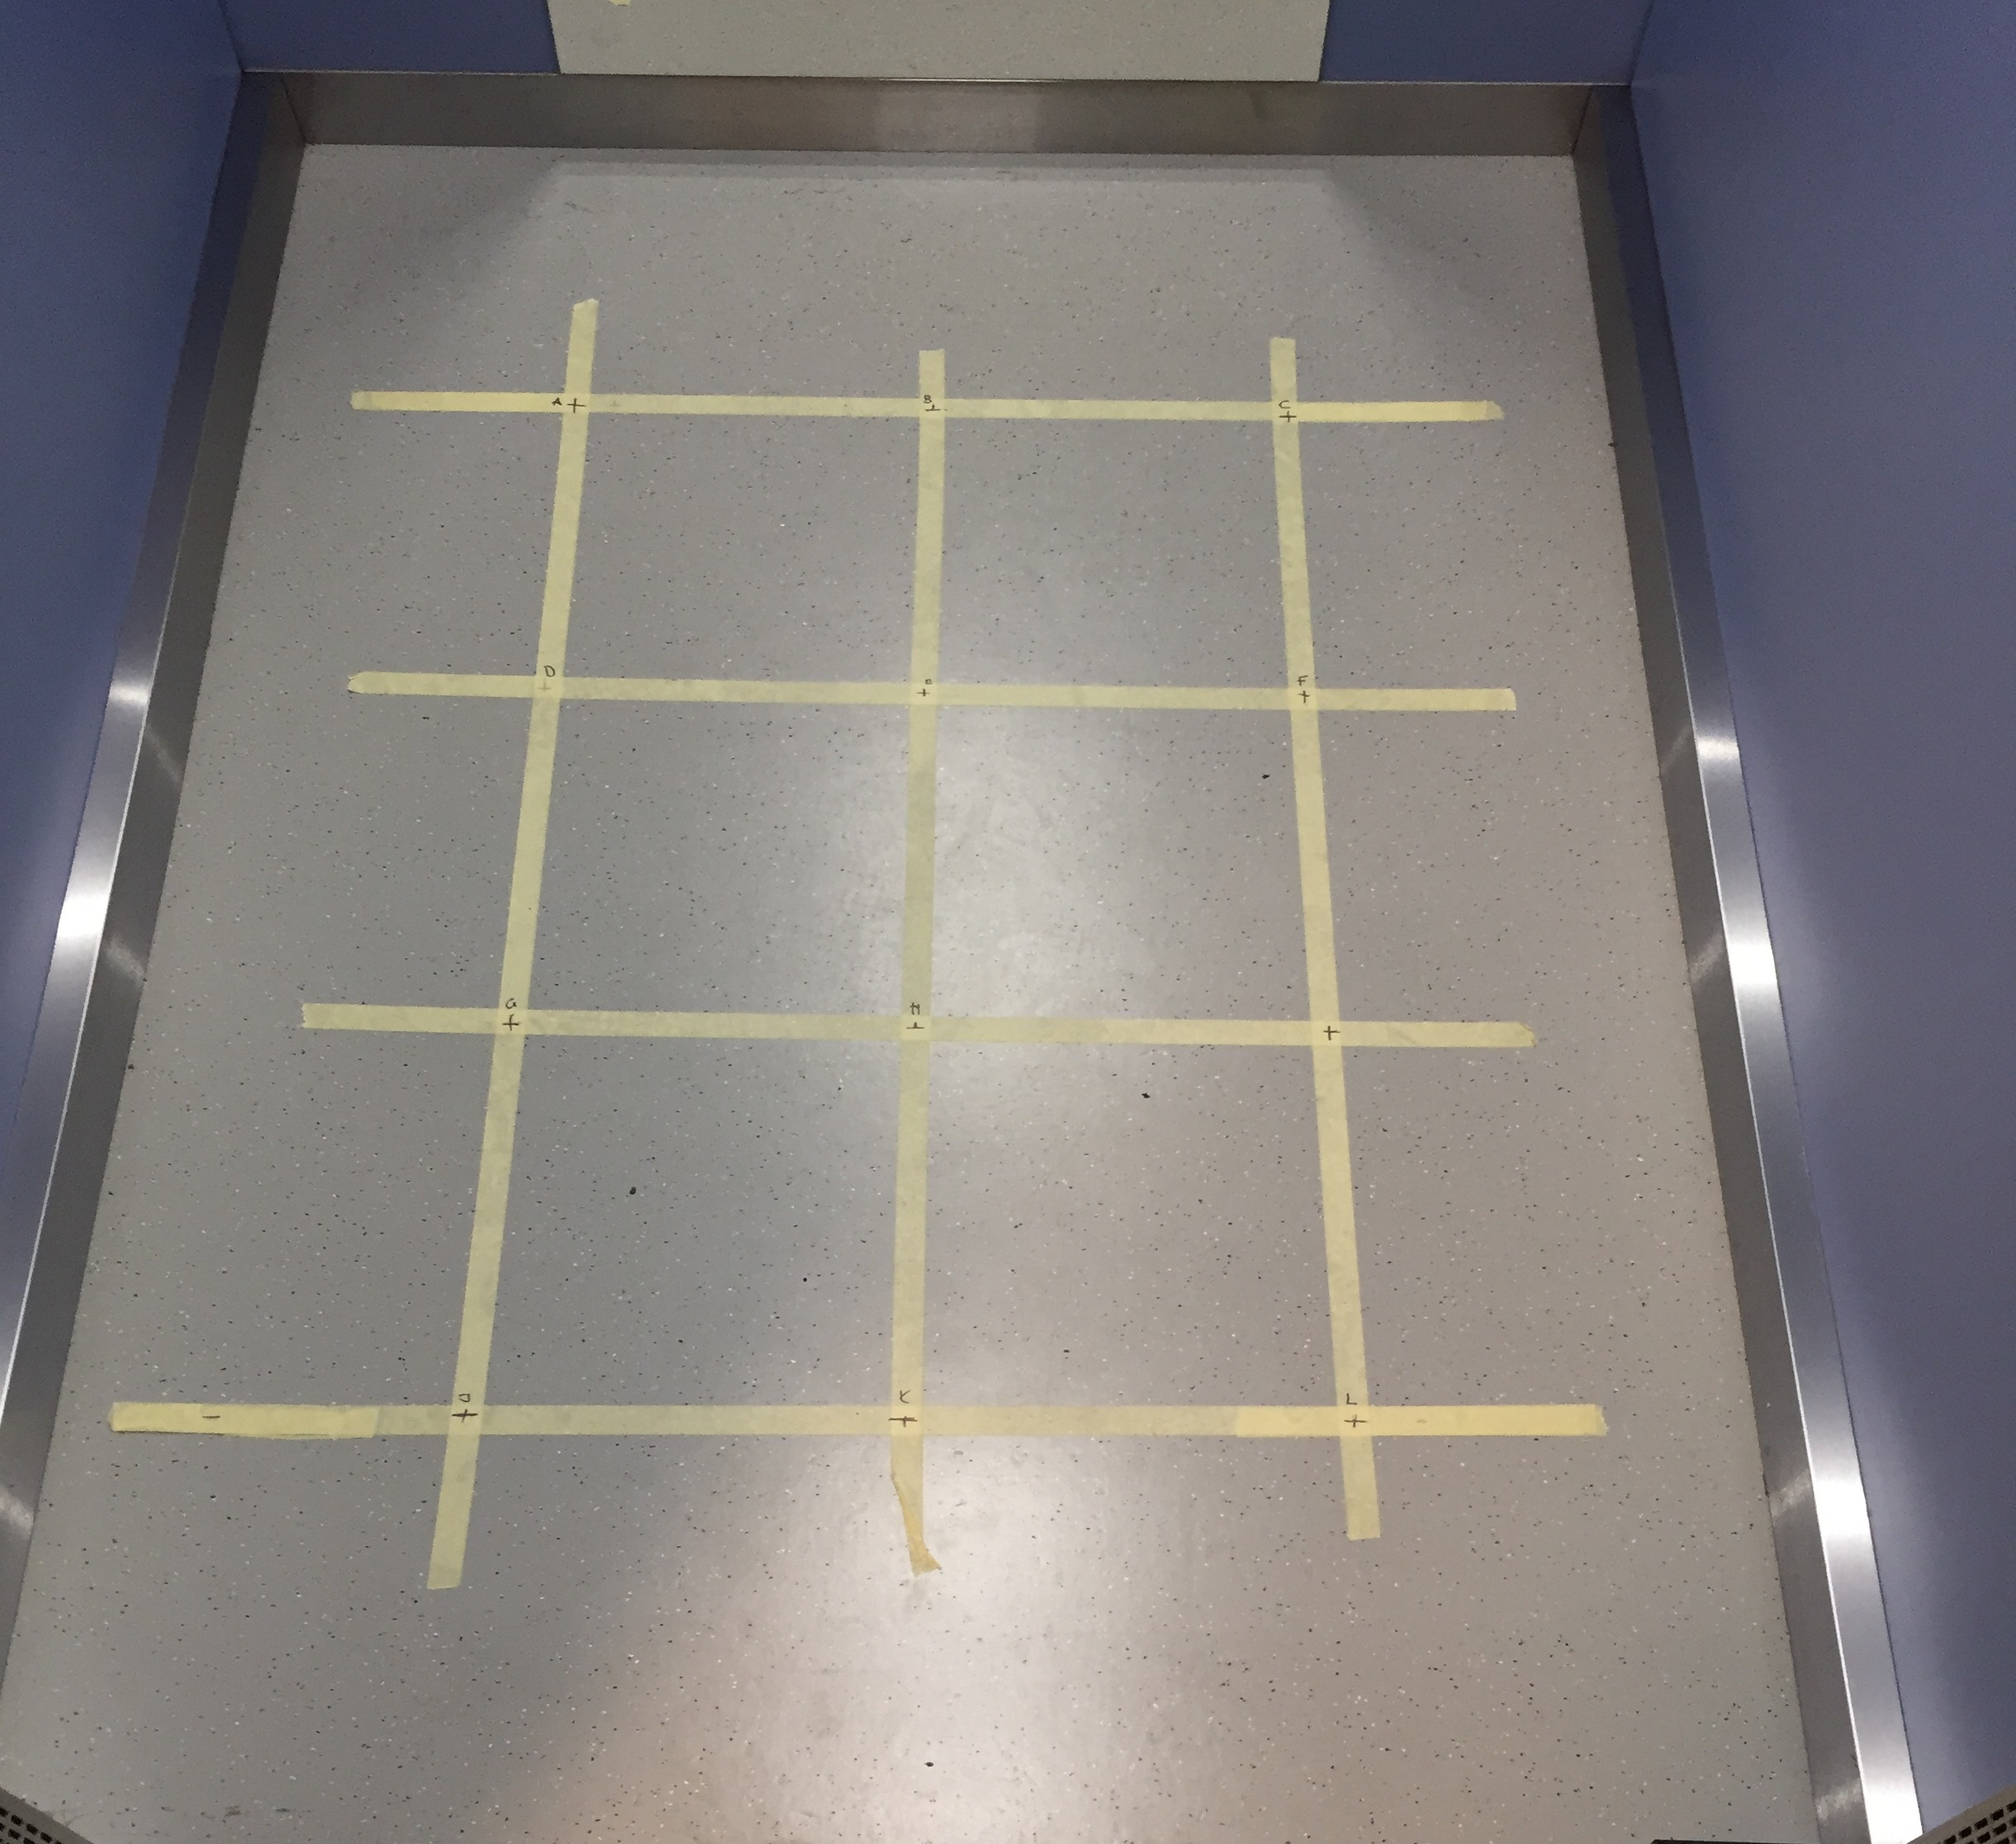
\includegraphics[width=1.0\textwidth, angle=0]{fig/Messraster.JPG}
	\caption{Messraster für Personenmessungen}[Messraster für Personenmessungen]
	\label{fig:p1gallpositionsmean}
\end{figure}

In den einzelnen Bildern ist ersichtlich, dass 

\section{Resultate}


\begin{figure}[H]
	\centering
	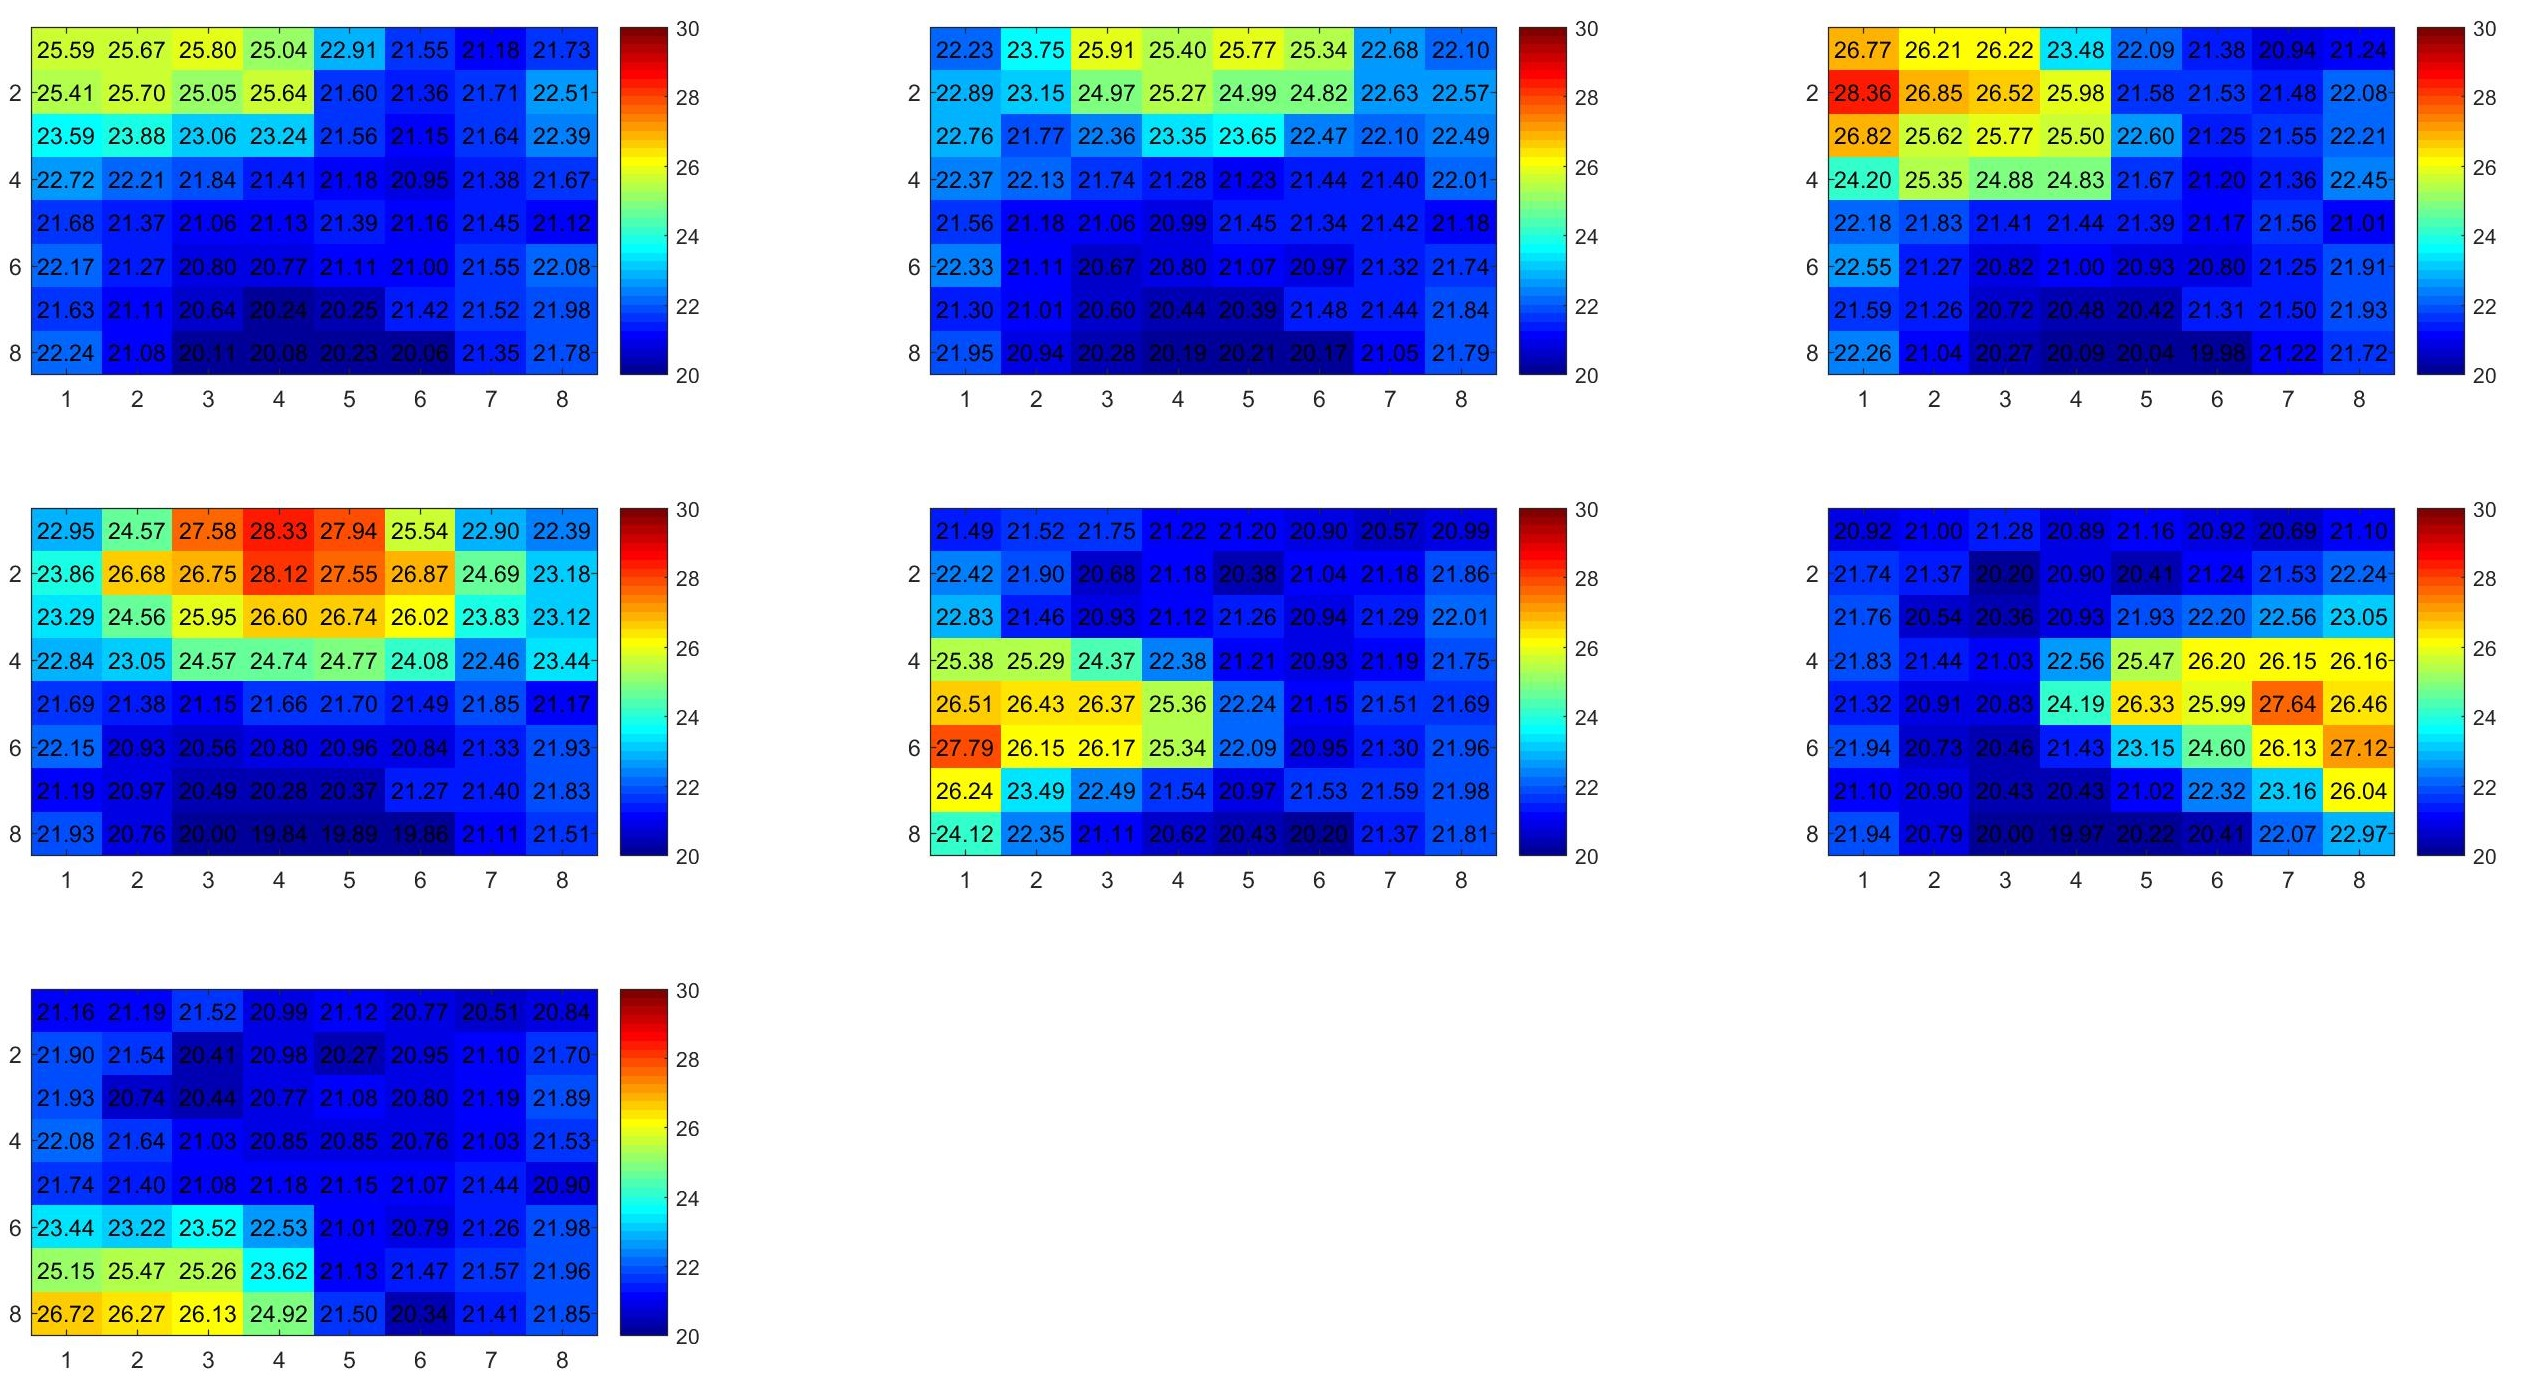
\includegraphics[width=1.0\textwidth]{fig/p1_g_Allpositions_mean}
	\caption[Mittelwerte Messung V1 Kategorie g]{Mittelwerte Messung V1 Kategorie g}
	\label{fig:p1gallpositionsmean}
\end{figure}

In den einzelnen Bildern ist ersichtlich, dass Personen im Zentrum leichter zu erkennen sind. Bei diesen Bilder wird der Kopf, der eine höhe Temperatru aufweist gemessen und daher


\begin{figure}
	\centering
	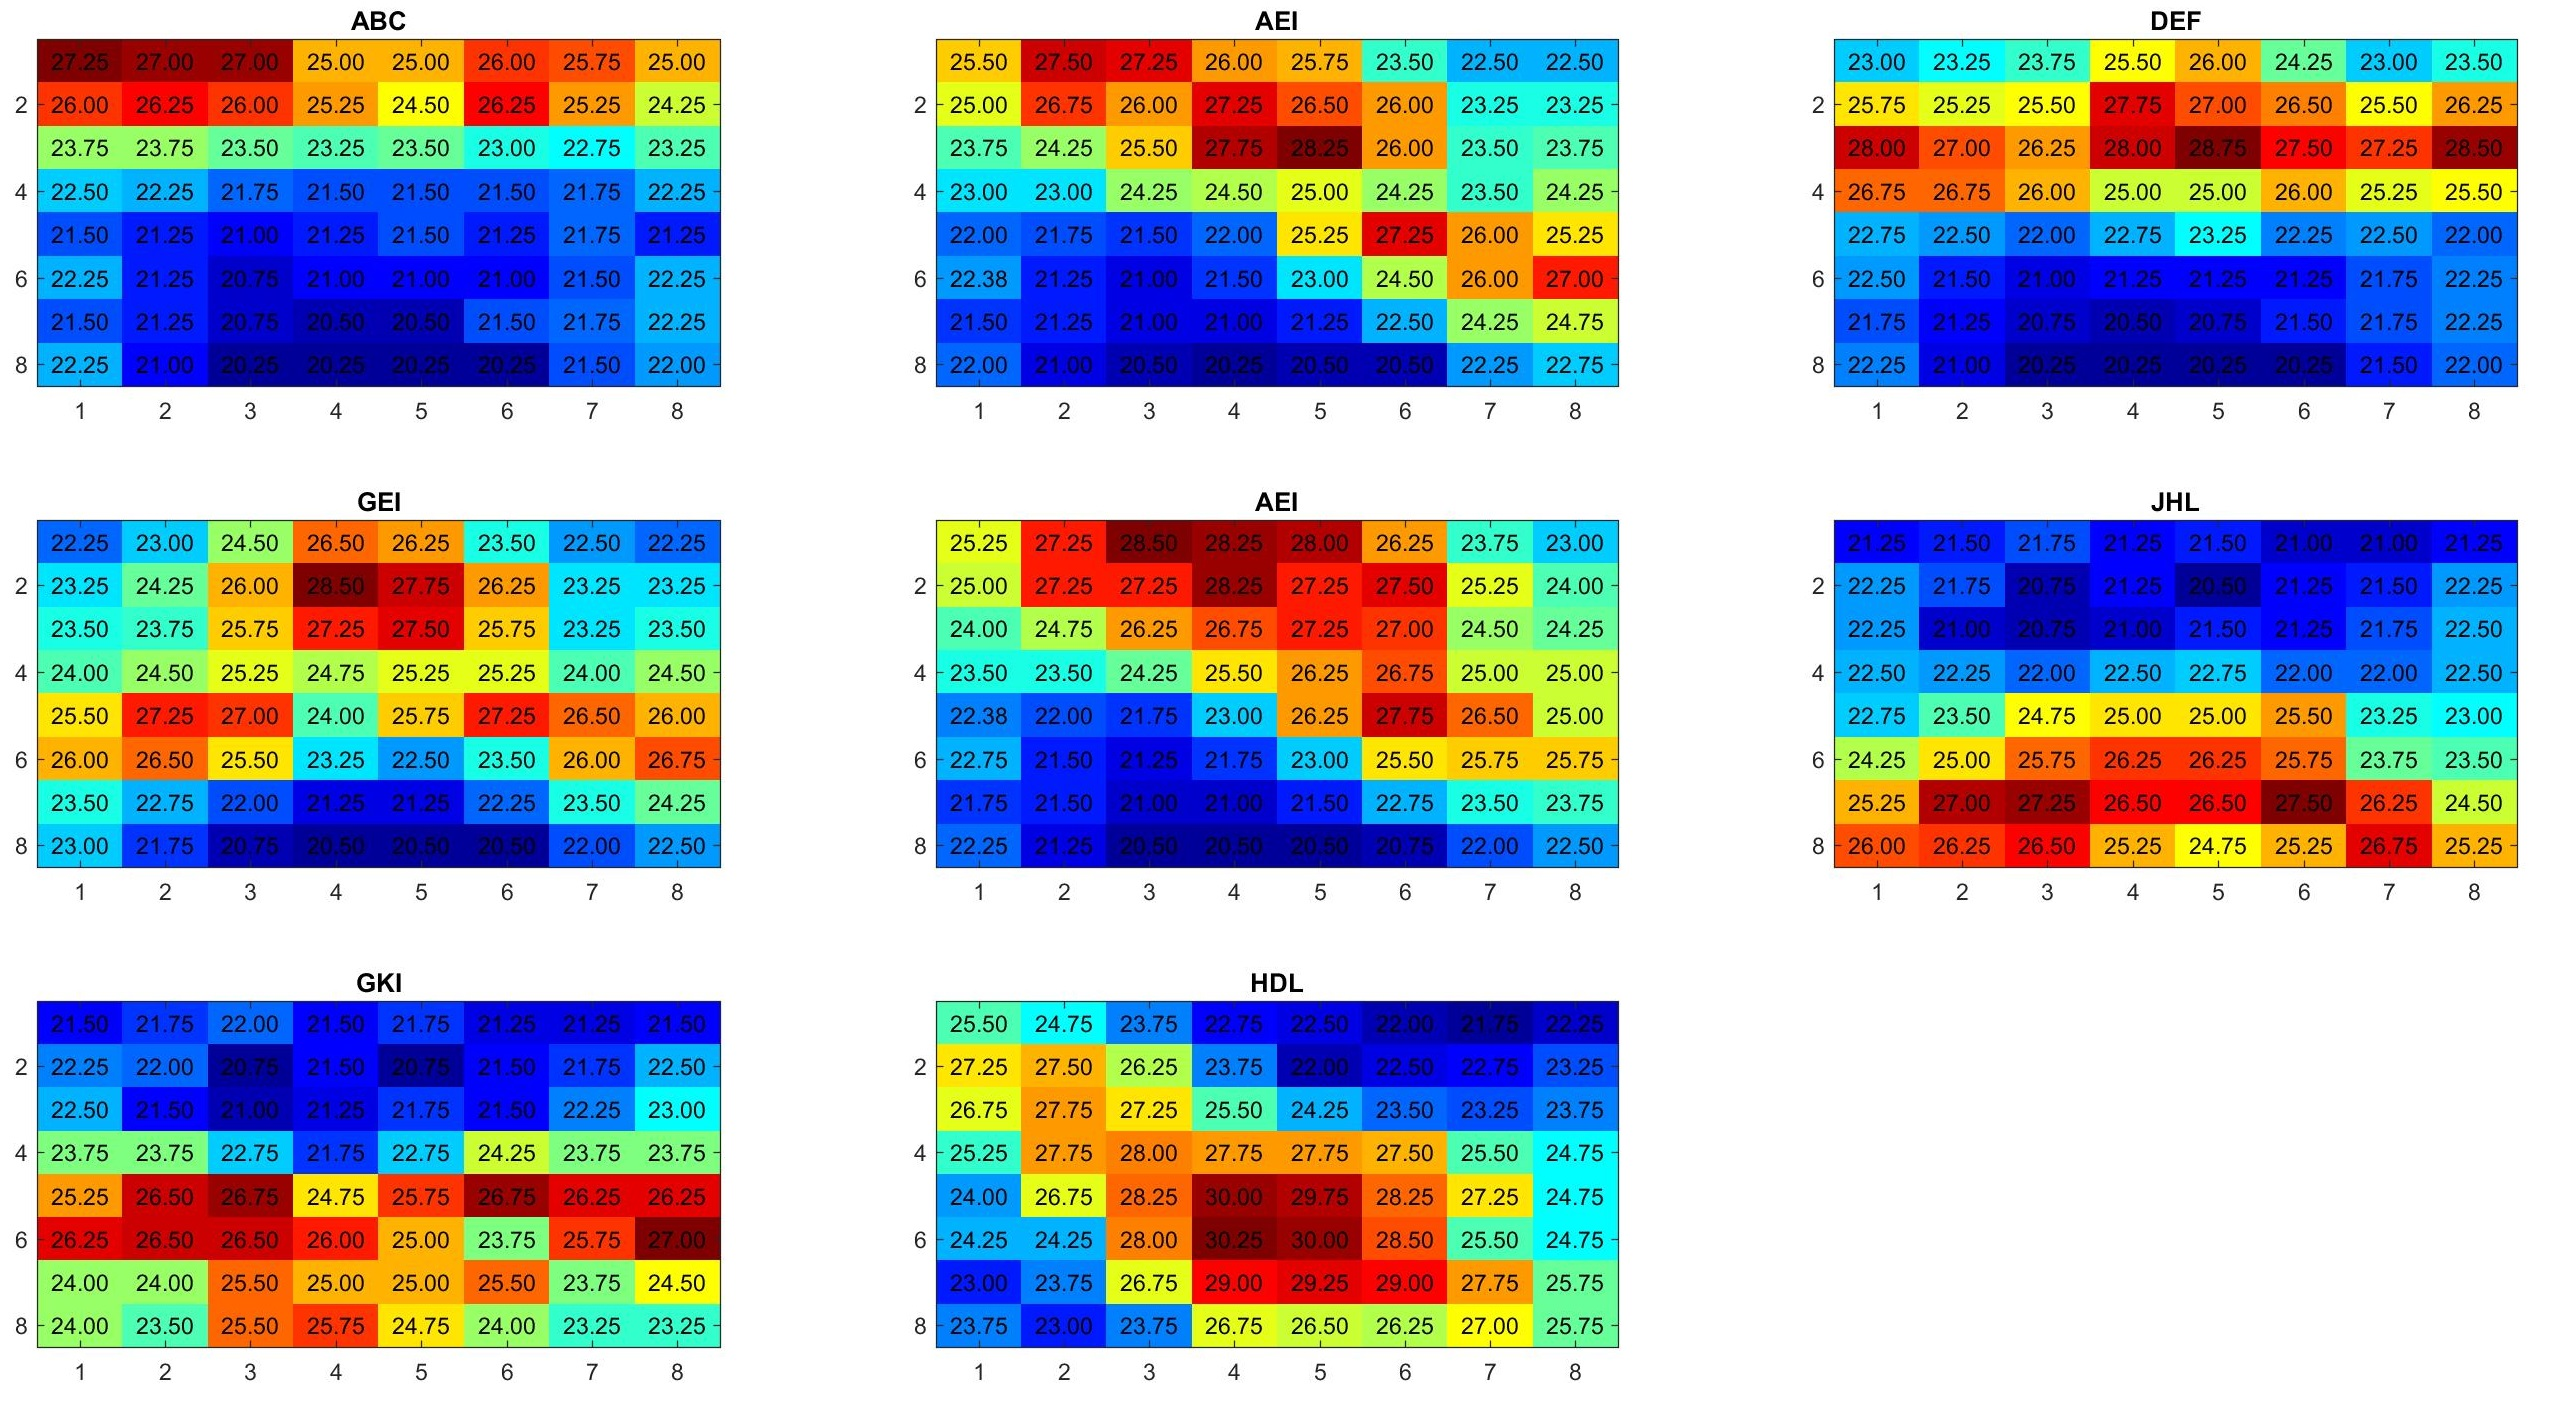
\includegraphics[width=1.0\linewidth]{fig/p3_3x3_allpositons}
	\caption{}
	\label{fig:p33x3allpositons}
\end{figure}





\section{Fazit}
Die Messresultate haben die Ergebnisse aus dem Kapitel \ref{chap:Informationsbeschaffung} bestätigt. Bei der Personenmessungen liegt die Schwierigkeit bei der Profilbildung von Personen. Da unterschiedliche Umgebungstemperaturen.
Es liegt nahe für dieses 
